\documentclass[revision-guide.tex]{subfiles}


%% Current Author: SEQ
\setcounter{chapter}{10}
\begin{document}
\tikzset{
  every pin/.style={
      font=\scriptsize,
      pin distance=4ex},
  small dot/.style={
      fill=gray,
      circle,
      scale=0.1}
}
\chapter{Oscillations}
\section{Simple Harmonic Motion}
\spec{Recall the condition for simple harmonic motion and hence identify situations in which simple harmonic motion will occur}


Any oscillation where the acceleration is proportional to the displacement from an equilibrium position and in the opposite direction to the displacement is described as Simple Harmonic Motion (SHM).

These two conditions can be expressed in equation form as:
\[ a \propto -x \]
Notice the minus sign to signify that the acceleration is in the opposite direction to the displacement.

We will mainly be looking at idealised springs and pendulums to understand the maths behind it but the real reason for studying SHM is that it is an excellent approximation for many of the oscillations that we come across in the natural world.

So while the topic is introduced with some rather prosaic examples this provides the building blocks to understanding earthquakes or how atoms vibrate in lattices as well as any musical instrument you can think of.

%\pagebreak

So without further ado let's look at our first and perhaps simplest example.

A mass on a spring on a smooth horizontal surface.
\vspace{0.2in}


\begin{tikzpicture}
\node[rectangle,scale = 1.8, fill=blue,inner sep=2.5mm, text = white] (a) at (3.75,3) {$m$};


\draw[decoration={aspect=0.3, segment length=2mm, amplitude=3mm,coil},decorate] (0,3) -- (a); 

\fill [pattern = north east lines] (0,2) rectangle (6,2.4);
\fill [pattern = north east lines] (-.5,2) rectangle (0,4);
\draw[thick] (0,2.4) -- (6,2.4);
\draw[thick] (0,2.4) -- (0,4);

\end{tikzpicture}

What happens if we move the mass by a distance x and then let it go?

\begin{tikzpicture}
\node[rectangle,scale = 1.8, fill=blue,inner sep=2.5mm, text = white] (a) at (5,3) {$m$};




\draw[decoration={aspect=0.3, segment length=3mm, amplitude=3mm,coil},decorate] (0,3) -- (a); 

\fill [pattern = north east lines] (0,2) rectangle (6,2.4);
\fill [pattern = north east lines] (-.5,2) rectangle (0,4);
\draw[thick] (0,2.4) -- (6,2.4);
\draw[thick] (0,2.4) -- (0,4);
\draw[thick, |-latex] (3,3.5) -- (4.25,3.5);
\node at (3.5,3.7) {$x$};
\end{tikzpicture}


Before going into any mathematical detail we can think about what will happen to the mass.
\begin{itemize}
\item We know that there is now a force from the stretched string which is pulling the mass back to its original position. 
\item This will cause the mass to accelerate to the left. 
\item Once the mass reaches its starting point it will overshoot and start compressing the spring.
\item This creates a resultant force which will again restore the mass to its original position.
\item This will cause the mass to accelerate to the right.
\item The mass will overshoot again and the cycle will continue.
\end{itemize}
Note that the direction of the acceleration is always opposite to the displacement.

The mathematical treatment for this starts very simply with a basic knowledge of Hooke's law.

The force on a stretched or compressed spring is given by 
\[
F=-kx
\]
where k is the spring constant.

Newton's second law tells us that 
\[
F=ma
\]

Putting these together we get
\[
a = \dfrac{F}{m}=-\dfrac{k}{m}x
\]
Because k and m are constant this satisfies the condition for SHM,
\[
a \propto -x
\]

\begin{example}
A  2kg mass attached to a horizontal spring of spring constant 0.3Nm$^{-1}$ is stretched by 10cm and then released.

Find the maximum acceleration of the mass


	\vspace{1cm}

		

		\textbf{Answer}

Using the formula $a = -\dfrac{k}{m}x$
The maximum acceleration will occur when x is a maximum so 
\[
acceleration_{max} = - \dfrac{0.3}{2} \times 0.1
\]
\[
acceleration_{max} = -0.015 ms^{-2}
\]

\end{example}






\spec{* show that the condition for simple harmonic motion leads to a differential equation of the form
\[ 
\dfrac{d^2x}{dt^2} = - \omega^2 x
\]
and that 
\[ 
x = A cos \omega t 
\] 
is a solution to this equation}


Acceleration is the rate of change of velocity 

\[
a = \dfrac{dv}{dt} 
\]

and velocity is the rate of change of displacement

\[
v = \dfrac{dx}{dt} 
\]

Putting these two together gives the condition for simple harmonic motion as.

\[
\dfrac{d^2x}{dt^2}=-\omega ^2 x
\]

where $\omega ^2$ is a (strange choice of) constant.

This is a second order differential equation and to solve it we need to find a function which when differentiated twice gives us the negative of the original function.

By inspection we can see that functions with $\sin \omega t$ and $\cos \omega t$ are both possible solutions.

e.g.

\begin{align*} 
x &= A cos \omega t \\
\dfrac{dx}{dt} &= - A\omega sin \omega t \\
\dfrac{d^2x}{dt^2} &= -A\omega^2 cos \omega t = -\omega ^2 x \\
\end{align*}

So $x= Acos \omega t$ is a solution (using sin is equivalent but with a phase offset.)

Looking at this function we can see that it will give us a cosine wave with an Amplitude of A and a time period of $ \dfrac{2 \pi}{\omega}$.

This gives us a frequency on $\dfrac{1}{T} = \dfrac{\omega}{2 \pi}$

So $\omega$ is the angular frequency (which explains our strange choice of constant).

\begin{tikzpicture}
	%curve
		\draw (0.5,1) cos (1.5,0) sin (2.5,-1) cos (3.5,0) sin (4.5,1) cos
			(5.5,0) sin (6.5,-1) cos (7.5,0) sin (8.5,1) cos (9.5,0)
			sin (10.5,-1) cos (11.5,0);
	% zero crossing
		\draw[dotted] (0.5,0) -- (11.5,0);
	%axis + labels
		\draw [<->] (0.5,1) -- (0.5,-1);
		\draw [->] (0.5,0) -- (11.5,0);
		\node at (11.7,0) {$t$};
		\node at (0.5,1.2) {$+A$};
		\node at (0.5,-1.2) {$-A$};
		\node at (0.3,0) {$0$};
	%Time period description
		\draw [<->] (4.5,1.15) -- (8.5,1.15);
		\node at (6.5,1.6) {Time period, $\dfrac{2 \pi}{\omega}$};
	%Amplitude description
		\draw [<->] (6.5,0) -- (6.5,-1);
		%to stop line overlap
		\draw [fill=white,ultra thick,white] (7,-0.3) rectangle (9,-0.7); 
		\node at (8, -0.5) {Amplitude, $A$};
\end{tikzpicture}

We now have a general expression for the displacement x of the object after a time t.

The value of $\omega$ will be given by the physical properties of the system.

e.g.
For the mass on a spring we looked at earlier

\begin{align*} 
F &= -kx && \text {Force on mass by Hooke's Law}\\
a &= -\dfrac{k}{m} x  && \text{gives acceleration}\\
\dfrac{d^2x}{dt^2} &= -\omega ^2 x && \text{comparing with condition for SHM} \\
\omega ^2 &= \dfrac{k}{m} && \text{gives value for constant } \omega \\
\omega &= \sqrt{\dfrac{k}{m}} \\
\end{align*}

\spec{* use differential calculus to derive the expressions
\[
v=-A \omega sin \omega t 
\] and 
\[a = -A\omega^2 cos \omega t 
\] 
for simple harmonic motion.}



This is achieved very simply by differentiating our expression for displacement with respect to time as velocity =$\dfrac{dx}{dt}$ and acceleration = $\dfrac{dv}{dt}$

Remember that the differential of cos is -sin.

so 
\[
x = A cos \omega t
\]
\[
v = \dfrac{dx}{dt}= -A \omega sin \omega t
\]
\[
a = \dfrac{dv}{dt}= -A \omega^2 cos \omega t
\]


\spec{ *recall and use the expressions $x = A cos\omega t, v = -A \omega sin \omega t, a = -A \omega^2 cos \omega t$ and $F = -m \omega^2x$ to solve problems}

We can use these equations to solve problems by identifying the variables and substituting.

The last equation is a combination of $a = -\omega^2 x$ and $F = ma$

\begin{example}


A mass attached to a spring is set into motion on a smooth horizontal surface. The amplitude of oscillation is 15mm and it takes 5 seconds to perform 20 oscillations.

Calculate the time period and frequency.

Hence calculate the velocity and acceleration after 9.3 seconds.

	\vspace{1cm}
    
\textbf{Answer}

The first part doesn't require any knowledge of SHM. If there are 20 oscillations in 5 seconds this means $\dfrac{20}{5}$ oscillations in one second.

So $f=4Hz$

and $T = \dfrac{1}{f} = 0.25s$

Now that we have the frequency we can calculate the angular frequency $\omega = 2 \pi f = 8 \pi$

We are given the amplitude A as 15mm and the time is 9.3 seconds so we can now use our SHM formulae.

So for the velocity

\[
v=-A \omega sin \omega t 
\]

\[
v = -15 \times 8 \pi sin (8 \times \pi \times 9.3)
\]
\[
v = -360 mms^{-1} = .36ms^{-1}
\]

and for acceleration

\[
a = \dfrac{dv}{dt}= -A \omega^2 cos \omega t
\]

\[
a = 15 (8 \times \pi)^2 cos (8 \times \pi \times 9.3)
\]

\[
a = 2900 mms^{-2} = 2.9ms^{-2}
\]


\end{example}



\spec{ recall and use $T = \dfrac{2 \pi}{\omega}$
as applied to a simple harmonic oscillator}

Angular frequency $w$ is how many radians per second the oscillator goes through with one complete cycle being $2 \pi$ radians.

So $\dfrac{1}{\omega}$ is how many seconds is takes to complete one radian.

and the time for one complete cycle is $T = \dfrac{2 \pi}{\omega}$


\spec{ understand the phase differences between displacement, velocity and acceleration in simple harmonic
motion}

Plotting the equations \[x = A cos \omega t
\]
\[
v =  -A \omega sin \omega t
\]
\[
a = -A \omega^2 cos \omega t
\]
onto a graph gives the following.




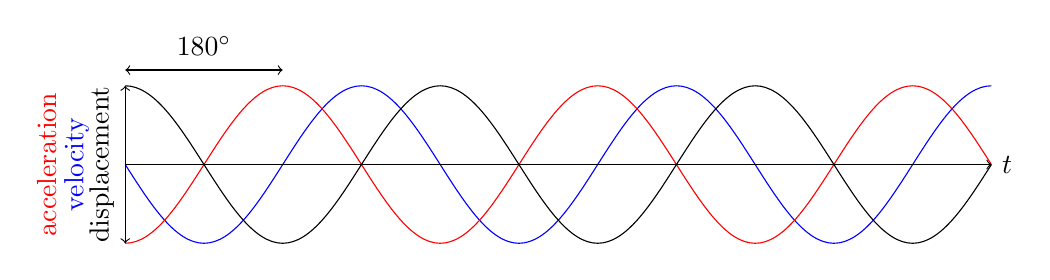
\begin{tikzpicture}
	%curve 1
		\draw[blue] (0.5,0) sin (1.5,-1) cos (2.5,0) sin (3.5,1) cos (4.5,0) 
			sin (5.5,-1) cos (6.5,0) sin (7.5,1) cos (8.5,0) sin (9.5,-1) 
			cos (10.5,0) sin (11.5,1);
	%curve 2
    \draw[red] (0.5,-1) cos (1.5,0) sin (2.5,1) cos (3.5,0) sin (4.5,-1) cos
			(5.5,0) sin (6.5,1) cos (7.5,0) sin (8.5,-1) cos (9.5,0)
			sin (10.5,1) cos (11.5,0);
		cos (10.5,0) sin (11.5,1);
    %curve 3
        	\draw (0.5,1) cos (1.5,0) sin (2.5,-1) cos (3.5,0) sin (4.5,1) cos
			(5.5,0) sin (6.5,-1) cos (7.5,0) sin (8.5,1) cos (9.5,0)
			sin (10.5,-1) cos (11.5,0);
	% zero crossing
		\draw[dotted] (0.5,0) -- (11.5,0);
	%axis + labels
		\draw [<->] (0.5,1) -- (0.5,-1);
		\draw [->] (0.5,0) -- (11.5,0);
		\node at (11.7,0) {$t$};
		\node[rotate=90] at (0.2,0) {displacement};
        \node[rotate=90, blue] at (-0.12,0) {velocity};
        \node[rotate=90, red] at (-0.5,0) {acceleration};
	%Phase difference description
		\draw [<->] (0.5,1.2) -- (2.5,1.2);
		\node at (1.5,1.5) {$180^\circ$};
\end{tikzpicture}



Note the phase shift between displacement, velocity and acceleration.

Velocity is $\dfrac{\pi}{2}$ or $90^\circ$out of phase with displacement.

Acceleration is $\pi$ or $180^\circ$ out of phase with displacement.

So when acceleration or displacement has a maximum magnitude, the velocity is zero




\spec{ *show that the total energy of an undamped simple harmonic system is given by $E = \dfrac{1}{2}mA^2\omega^2$ and
recognise that this is a constant}

For an undamped system no energy is lost to the surroundings so the total energy is conserved.

The total energy will take the form of Potential Energy  and Kinetic Energy.

Considering our mass on a spring at maximum displacement the spring will be at maximum extension and the mass will be stationary. So the total energy will be in the form of P.E.

Similarly when the displacement is zero all the energy will be K.E.

At any point in between the total energy will be a mixture of K.E. and P.E. 

As the total energy is the same at any point we can pick what's easiest to derive an equation for it.

So at zero displacement.

\begin{align*} 
T.E. &= K.E. \\
&= \dfrac{1}{2}mv_{max}^2 \\
&= \dfrac{1}{2}mA^2\omega^2 \\
\end{align*}

\spec{ recall and use $E = \dfrac{1}{2}mA^2\omega^2$ to solve problems}

We can look at example problem to see how this works.


\begin{example}

A mass of 8kg is attached to a spring with a spring constant of $5 Nm^{-1}$ on a smooth horizontal surface.
It is pulled back a distance of 20 cm and then released. 

Calculate the total energy of the system, the time period of oscillation and the velocity of the mass when the displacement is 10 cm.


\end{example}





    
\textbf{Answer}

One way to approach this question is by using our equation for the energy stored in a spring.

\[
P.E = \dfrac{1}{2}kx^2
\]

\[
P.E = \dfrac{1}{2} \times 5 \times .2^2 = 0.1J
\]

We also know that all the energy at this point is in the form of potential as the mass is not moving so this is the total energy of the system and will not change.



For the time period we can first calculate the angular frequency using our energy equation.

\begin{align*} 
E = \dfrac{1}{2}mA^2\omega^2 &= 0.1 J\\
\therefore \omega &= \sqrt{\dfrac{2 E}{m A^2}}\\
&= \sqrt{\dfrac{2 \times 0.1}{8 \times 0.2^2}}\\
&= 1 rads^{-1}\\
\omega &= \dfrac{2 \pi}{T} \\
\therefore T &= 2 \pi = 6.2 seconds \\
\end{align*}


When the mass has a displacement of 10cm, the total energy will be the kinetic and potential energy.


\begin{align*} 
T.E. = P.E + K.E. &= 0.1J \\
 \dfrac{1}{2} \times 5 \times .1^2 + K.E. &= 0.1J\\
 0.025 + K.E. &= 0.1J  \\
 \implies K.E. &= 0.075J \\
 \dfrac{1}{2}mv^2 &= 0.075J \\
 v &= 0.17 ms^{-1} \\
 \end{align*}



\pagebreak

\spec{ distinguish between free, damped and forced oscillations}

A free oscillator is one which is set in motion and left to oscillate without any external forces or damping.

e.g. an ideal pendulum with no friction.

A forced oscillation is one where an external periodic force is applied. 

e.g. pushing a child on a swing.

Damping is where frictional forces remove energy from the system and the oscillations die down.

This can be increased intentionally for example adding thick oil to car suspension to prevent you bouncing around every time the car hits a bump.

If a system is lightly damped it will gradually come to rest after a number of cycles. 

An important case is critical damping where the system comes to rest without overshooting and in the shortest possible time. 

 

\spec{ recall how the amplitude of a forced oscillation changes at and around the natural frequency of a system
and describe, qualitatively, how damping affects resonance.}

Every system has a natural frequency of oscillation which will depend on its physical properties. In the case of a mass on a spring it will depend on the mass and spring constant but more complex examples e.g. washing machines or the millennium bridge will also have natural frequencies.

If we apply a driving force to an oscillator, the effect it has will depend on the amplitude of the driving force and its frequency compared to the natural frequency of the system. 

For a simple example try holding a spring with a mass on the end of it and move your hand up and down rhythmically.

If you move your hand very slowly the spring won't stretch or contract and the mass will simply follow the movement of your hand. So the amplitude will be the same as the amplitude of the driving frequency.

As you start to increase the frequency of your hand movement the spring will start to stretch and contract and the mass will move more than your hand. So the amplitude of oscillation increases.

Once the frequency of your hand is close to the natural frequency you are adding energy at just the right point in the cycle to increase the amplitude with each cycle and the amplitude gets very large. We call this resonance.

If we know move our hand with a very high frequency, the spring stretches and compresses but the mass doesn't much have time to accelerate hence the amplitude starts to get very small.


\begin{itemize}
\item Low frequency driving force, amplitude of oscillator = amplitude of driver.
\item Driving frequency around natural frequency, resonance - very high amplitude oscillations.
\item High frequency driving force, low amplitude oscillations.
\end{itemize}



In the real world we need to consider damping which will affect all systems to some degree. Damping will come from frictional forces and will remove energy from the system every cycle. If the energy added by the driving force is more than is removed by damping then the amplitude will increase. As the amplitude increases, the energy removed each cycle will also increase until a maximum amplitude is reached.

From this it is clear that the more damping there is, the lower the amplitude. 

Another feature is that as we have more damping, the frequency at which resonance occurs is less. You can think of this as damping slowing down the system and so reducing the natural frequency (although strictly speaking the natural frequency refers to an undamped system).


This is all expressed in the following graph where I have used the damping ratio $\zeta$ as a measure of how much damping there is. Its not on the syllabus, you will only need to know qualitatively how damping affects resonance e.g. light damping and heavy damping but I though it would be good to introduce you to another Greek letter.


\begin{tikzpicture}
  \begin{axis}[
    % labels
    tick label style={font=\scriptsize},
    xlabel={Driving Frequency},
    ylabel={Amplitude / Driving Amplitude},
    ytick={0,1,2,3,4,5},
    xtick={0,1,2,3},
    xticklabels={0,$\omega_\mathrm{f}$,,},
    %
    % plot lines property
    no markers,
    line width=0.3pt,
    cycle list={{black,solid}},
    %
    % dominio 2D
    samples=200,
    smooth,
    domain=0:2.5,
    xmin=0, xmax=2.5,
    ymin=0, ymax=5.0,
    %
    % canvas dimensions
    width=12cm, height=12cm
    ]

    % horizontal help line
    \draw[help lines] (axis cs:0,1) -- (axis cs:2.5,1);
    % vertical help line
    \draw[help lines] (axis cs:1,0) -- (axis cs:1,5);

    % draw curves
    \addplot {1/sqrt((1-x^2)^2+4*0.05^2*x^2)};
    \addplot {1/sqrt((1-x^2)^2+4*0.10^2*x^2)};
    \addplot {1/sqrt((1-x^2)^2+4*0.20^2*x^2)};
    \addplot {1/sqrt((1-x^2)^2+4*0.30^2*x^2)};
    \addplot {1/sqrt((1-x^2)^2+4*0.40^2*x^2)};
    \addplot {1/sqrt((1-x^2)^2+4*0.50^2*x^2)};
   % \addplot {1/sqrt((1-x^2)^2+4*1.00^2*x^2)};
   % \addplot {1/sqrt((1-x^2)^2+4*2.00^2*x^2)};

    % draw maximum curve
    \addplot[dashed,domain=0:0.99] {1/sqrt(1-x^4)};

    %  curve labels
    \node[small dot,pin=30:{$\zeta_0=0{,}05$}] at
      (axis cs:1.10,4.22) {};
    \node[small dot,pin=30:{$\zeta_0=0{,}10$}] at
      (axis cs:1.10,3.29) {};
    \node[small dot,pin=30:{$\zeta_0=0{,}20$}] at
      (axis cs:1.10,2.05) {};
    \node[small dot,pin=30:{$\zeta_0=0{,}30$}] at
      (axis cs:1.20,1.19) {};
    \node[small dot,pin=30:{$\zeta_0=0{,}40$}] at
      (axis cs:1.28,0.83) {};
    \node[small dot,pin=30:{$\zeta_0=0{,}50$}] at
      (axis cs:1.50,0.51) {};

   % \node[small dot,pin=210:{$\zeta_0=1{,}00$}] at
      (axis cs:0.52,0.79) {};
   % \node[small dot,pin=210:{$\zeta_0=2{,}00$}] at
      (axis cs:0.60,0.40) {};
  \end{axis}
\end{tikzpicture}


\begin{itemize}
\item At very low driving frequencies the amplitude is the same as the driving amplitude.
\item With low damping we get a sharp resonance peak.
\item More damping creates a broader resonance peak.

\item Increasing damping reduces the amplitude at all frequencies.

\item The resonance peak shifts lower with increased damping.


\item As the frequency gets very high the amplitude will tend to zero regardless of damping or driving amplitude.


\end{itemize}


\end{document}



%sagemathcloud={"latex_command":"latexmk -xelatex -f -g -bibtex -synctex=1 -interaction=nonstopmode '11-oscillations.tex'"}
